% Liu Pinxin, Task 2 personal report (compile with xelatex)
\documentclass[11pt,a4paper]{ctexart}

\usepackage[a4paper,margin=2.4cm]{geometry}
\usepackage{graphicx}
\usepackage{booktabs}
\usepackage{longtable}
\usepackage{array}
\usepackage{xcolor}
\usepackage{listings}
\usepackage{caption}
\usepackage{indentfirst}
\usepackage[hidelinks]{hyperref}

\setlength{\parindent}{2em}
\captionsetup{font=small,labelfont=bf}

\definecolor{codebg}{gray}{0.97}
\lstset{
  language=Python,
  basicstyle=\ttfamily\footnotesize,
  commentstyle=\color{gray},
  keywordstyle=\color{blue!70!black},
  stringstyle=\color{red!60!black},
  backgroundcolor=\color{codebg},
  frame=single,
  breaklines=true,
  numbers=left,
  numberstyle=\tiny\color{gray},
  numbersep=6pt,
  columns=fullflexible,
  keepspaces=true,
  showstringspaces=false,
}

\title{\heiti\Large Grasp Verification via Gripper State and Closing Time on the RoboMaster EP\\
       \normalsize Robot Integration Project, Task 2 --- Personal Experiment Report}
\author{\normalsize Member: Liu Pinxin \quad Focus: real-robot grasp verification\\
        \normalsize Student ID: 24020036042 \quad Date: September 2026}
\date{}

\begin{document}
\ctexset{abstractname = {Abstract}, figurename = {Figure}, tablename = {Table}}
\maketitle
\thispagestyle{empty}

\begin{abstract}
Task 2 asks the robot to do a fixed-point pick without vision: grab an object
at A, carry it to B, release, and go home. I was responsible for the gripper
verification module. The official SDK only reports two gripper states,
\texttt{normal} and \texttt{closed}, and they describe the mechanism's own
position, not whether an object is actually in the jaws: an empty close
passes through \texttt{normal} on the way down, a squeezed tennis ball can
also reach \texttt{closed}, and a rigid object wedged in the jaws stops them
at \texttt{normal}. During debugging I first removed a premature pause of the
status stream and replaced it with polling at 0.2\,s over the 5\,Hz stream,
then split ``how long the state has held'' and ``how fresh the messages are''
into two separate clocks, and finally used a power sweep to set the
thresholds: at power level 30, reaching \texttt{closed} within 2.0\,s of the
close command is taken as a successful grasp. Across five acceptance runs,
four runs with an object closed in 1.4/1.4/1.6/1.4\,s, were accepted and
carried through, and one deliberately empty close at 2.4\,s was rejected,
after which the cycle stopped and the arm returned to a safe pose. The sample
size is small, the thresholds must be re-swept for any new object, and
communication-failure cases remain untested.

\vspace{1em}
\noindent\textbf{Keywords:} RoboMaster EP; gripper state; grasp verification;
closing-time threshold; power sweep
\end{abstract}

\section{Task and My Role}

\subsection{Task Goal and Platform}
Task 2 is a fixed-point pick: the robot homes, moves above point A, lowers the
arm, closes the gripper on the object, lifts, turns to point B, releases, and
homes. No vision is used anywhere; the grasp point is guaranteed by table
markings and preset trajectory parameters. The platform was originally a
mechArm 270 and was replaced with a RoboMaster EP, a substitution the course
staff approved. The simulation side runs Gazebo with ROS 2, and the real robot
runs on a Jetson Orin NX driven by DJI's official RoboMaster SDK. Both sides
share one set of state topics and the same task sequence; switching platforms
only changes device, communication, and position configuration, never the
task logic. Before each round the operator re-places the object at A, clears
B, and restores the chassis to its marked initial heading; ``homing'' at the
end means wheel speed zero, arm back to its calibrated center or home pose,
and gripper open. The safe working height is 0.45\,m throughout, below the
0.5\,m ceiling. The team first got five full rounds working in simulation
(5/5 success, wall-clock 95.22\,$\pm$\,4.22\,s), and the real robot port
adapts parameters on top of that.

\subsection{Where My Module Sits}
The team has four members: Yan Jiahui owns the simulation model, Liu Yuchen
the five-round simulation flow, Gong Chengtian the real-robot motion
execution, and I own the gripper verification module on the real robot. The
module sits between ``gripper close'' and ``test lift'' in the action chain:
after the gripper closes, it returns accept (continue with the test lift and
the carry) or reject (stop the cycle and return to a safe pose), and only
then does the chain move on; its position is shown in
Figure~\ref{fig:chain}.

\begin{figure}[htbp]
\centering
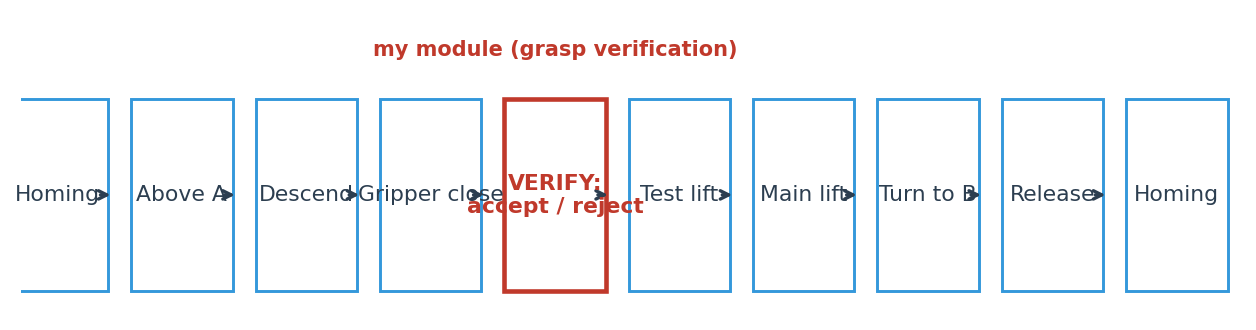
\includegraphics[width=0.95\linewidth]{figures/fig1_chain.png}
\caption{Position of the verification module in the pick chain (my part in red)}
\label{fig:chain}
\end{figure}

\begin{figure}[htbp]
\centering
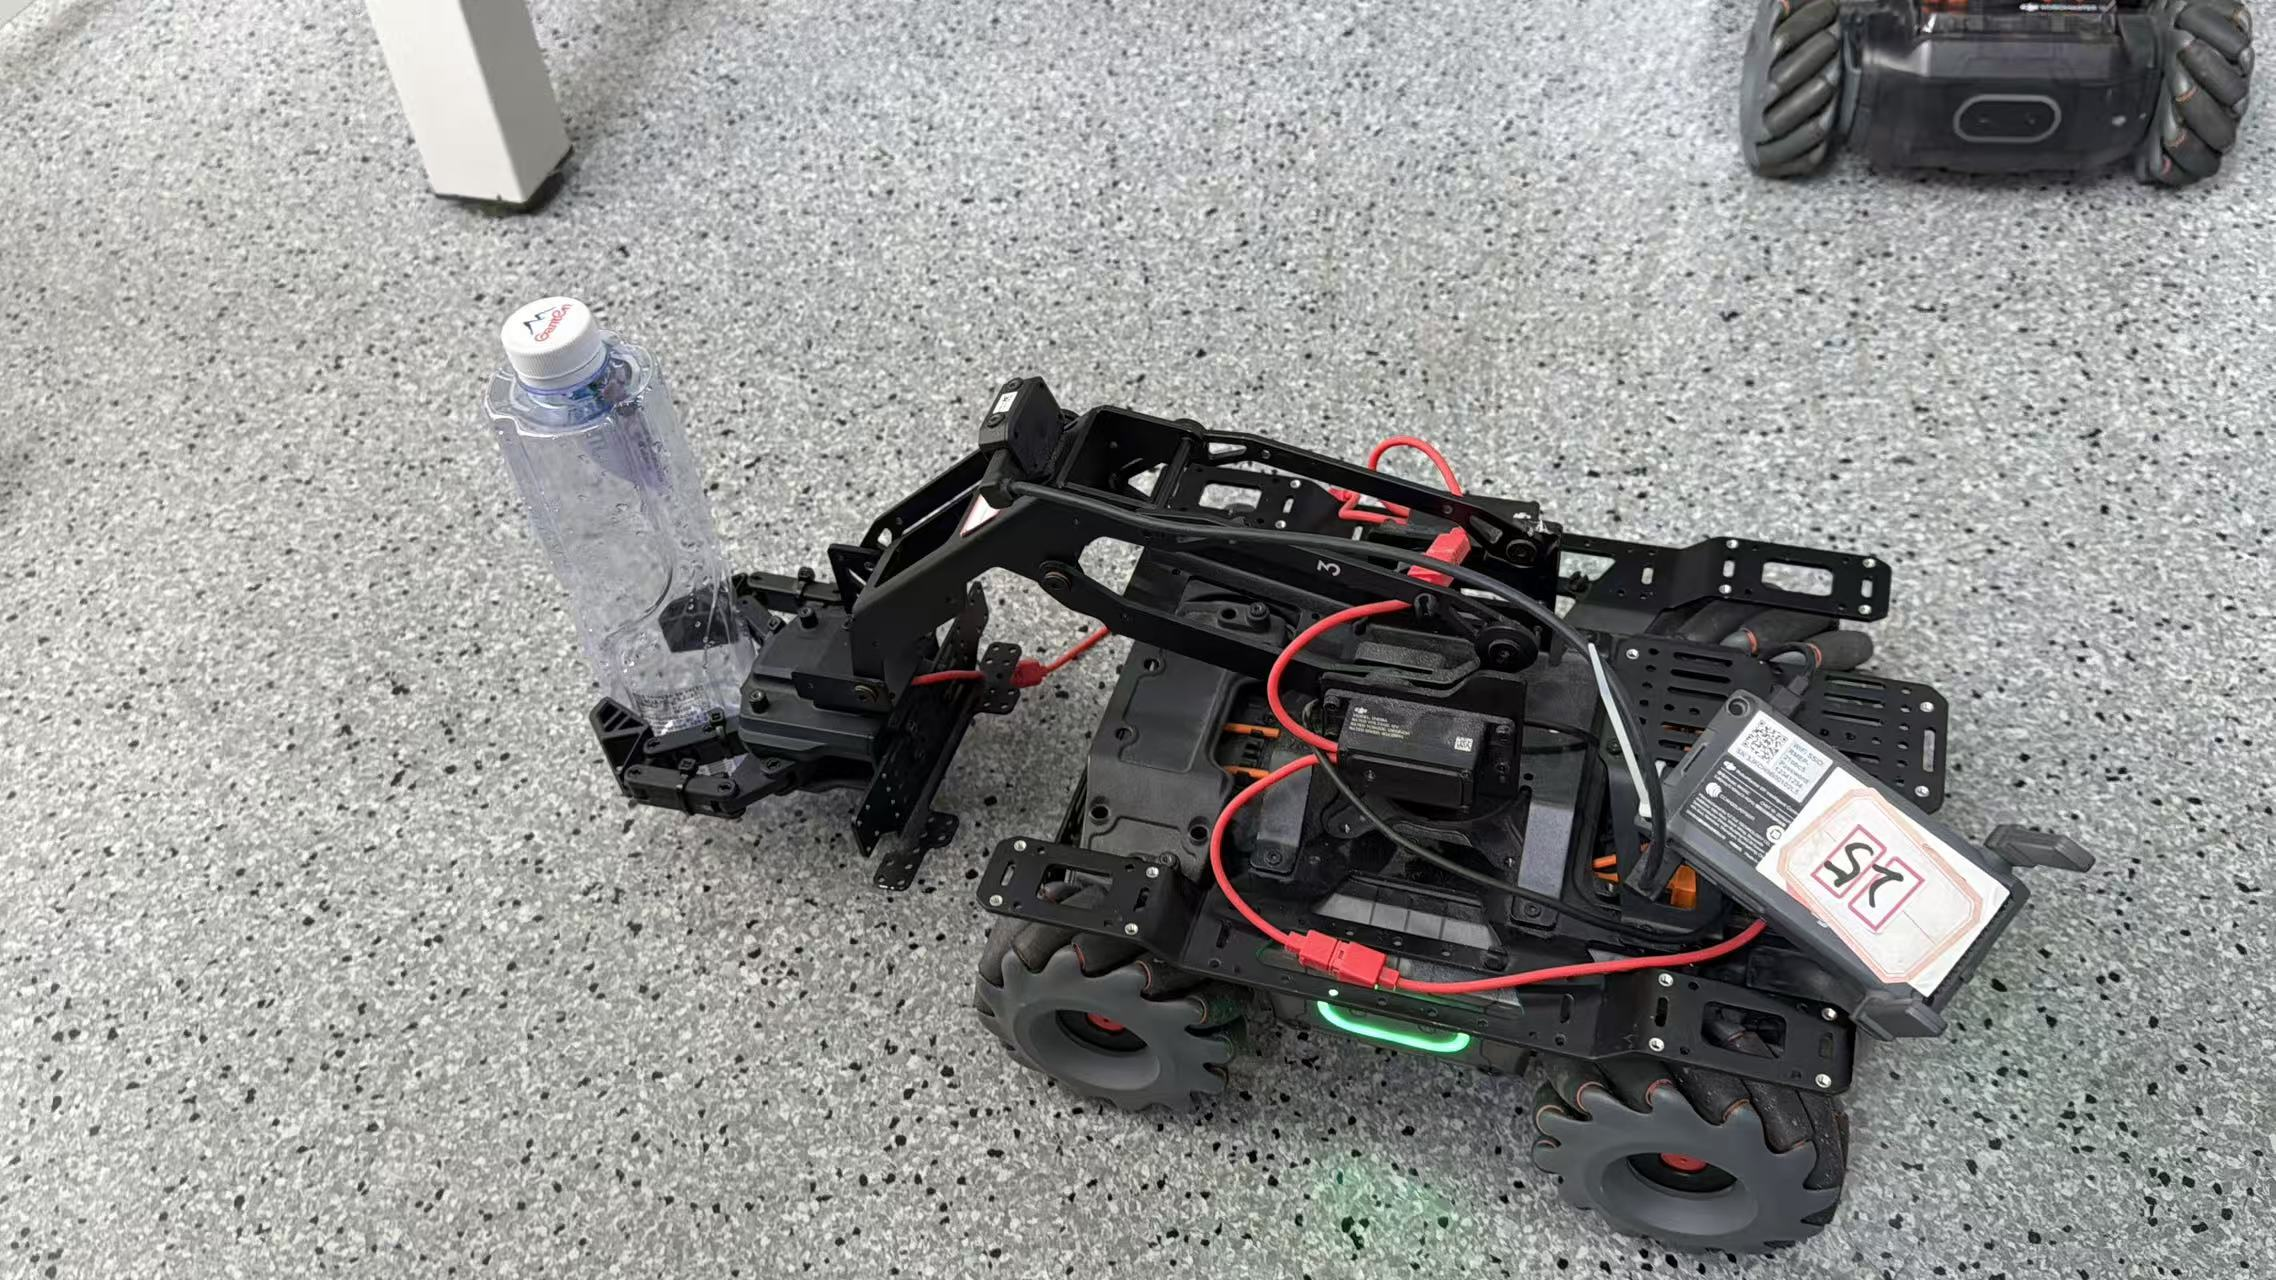
\includegraphics[width=0.92\linewidth]{photos/p1.jpg}
\caption{The real-robot experiment setup}
\label{fig:field}
\end{figure}

The module's inputs are the gripper state (\texttt{opened}/\texttt{normal}/
\texttt{closed}) pushed by the SDK at 5\,Hz together with each message's local
receive time; its output is accept/reject plus a reason string. The ground
truth comes from the ``object present or not'' annotation made before each
round, and from on-site video. One distinction matters here: what I deliver
is ``the judgment matches the ground truth'', not ``the carry succeeded''.
Gripper verification alone cannot prove the object ended up in B, and whether
the object actually rides up with the jaws after the test lift is still
confirmed by eye on site (Section 6 returns to this).

\section{Initial Misjudgments}

When I took over this module my plan was simple: \texttt{normal} means the
jaws stopped mid-way, \texttt{closed} means they reached the bottom, so one
of the two states must mean ``grasped''. The first real-robot run said
otherwise. The two SDK states describe the mechanism's own position, not
object presence:

\begin{itemize}\setlength{\itemsep}{2pt}
\item during an empty close the jaws briefly pass through \texttt{normal}, so
      a single \texttt{normal} observation mistakes an empty close for a
      grasp;
\item a squeezed tennis ball lets the jaws also reach \texttt{closed}, so
      \texttt{closed} alone cannot tell a soft-ball grasp from an empty close
      that bottomed out;
\item a rigid object (the block) wedged in the jaws stops them at
      \texttt{normal}, so ``grasped'' shows up as \texttt{normal} for rigid
      objects.
\end{itemize}

In other words, using any single state as the verdict is guaranteed to fail
on some rounds. On top of that I hit three concrete pitfalls, all visible in
the code and the commit history; Section 3 walks through them in the order
they happened.

\section{How the Criterion Evolved}

\subsection{Pitfall 1: pausing mid-close froze the status stream (commit \texttt{907c028})}
On the afternoon of 10 September I wrote the first version of the judgment
(commit \texttt{6f5b743}): after issuing the close command it waited for a
state, and during that wait it called the SDK's pause interface once to save
resources. On the robot that evening every judgment got stuck on stale
values: the push stream was frozen during the close, so everything read
afterwards was out of date. At 19:32 I removed the pause and switched to
polling every 0.2\,s (commit \texttt{907c028}), so the state keeps flowing
for the whole close. The lesson stuck with me: never turn off the very data
channel your judgment is waiting on.

\subsection{Pitfall 2: transient \texttt{normal} during an empty close (commit \texttt{dd14b7f})}
With polling in place the next problem appeared immediately: in an empty-close
round, the moment the jaws passed through \texttt{normal} mid-travel got
judged as ``grasped'', and the chain went on to carry nothing. At 19:53 I
changed the criterion to a stable window (commit \texttt{dd14b7f}):
\texttt{normal} only counts if it holds for 2.5\,s continuously; a flash
does not count.

\subsection{Pitfall 3: the stable timer kept counting after the stream died}
The stable window exposed a third problem. The debug logs once showed the
``state stable'' timer still climbing while the jaws on the desk had long
stopped moving: the push stream had died, and the program kept extrapolating
from the timestamp of the last message. So I split the two clocks
(Figure~\ref{fig:clock}): one measures how long the state value has held,
reset only when the value changes; the other measures message freshness, the
receive time of the last push. The \texttt{normal}-stable branch now requires
both at once, and freshness older than 1.0\,s disqualifies the state.

\begin{figure}[htbp]
\centering
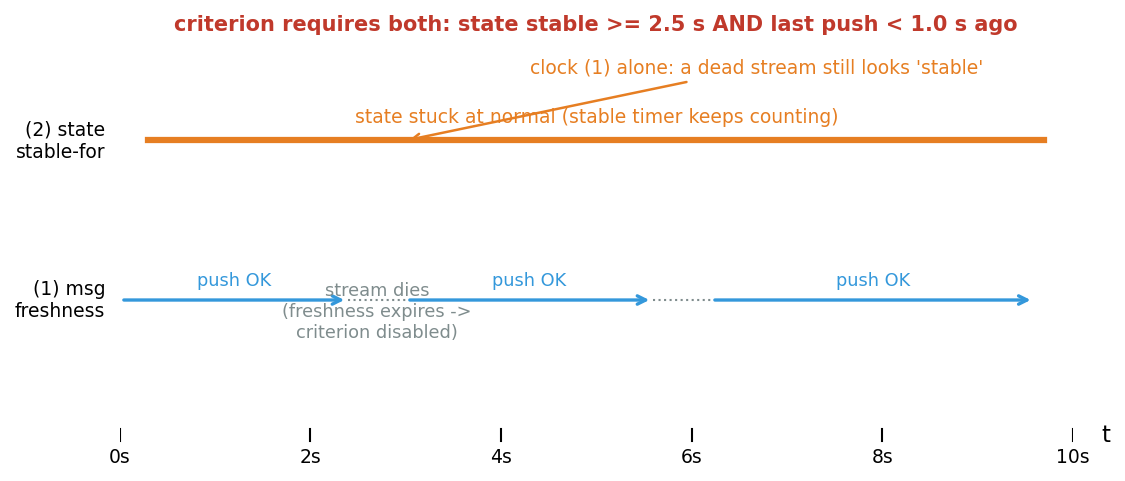
\includegraphics[width=0.9\linewidth]{figures/fig4_dual_clock.png}
\caption{Splitting state-hold time from message freshness: a dead stream can no longer fake stability}
\label{fig:clock}
\end{figure}

\subsection{Where the thresholds came from: the power sweep (commits \texttt{8d6548c}, \texttt{7ecd31d})}
One question remained: ``how fast is fast'' cannot be pulled from thin air.
I wrote a sweep probe (commit \texttt{8d6548c}) that, for each of the five
power levels 60/30/20/10/5, ran two trials --- an empty close and a close on
a tennis ball --- and recorded the time to first \texttt{normal}, the time to
first \texttt{closed}, and the final state; results are saved to the desktop
with timestamped filenames (commit \texttt{a9d6afc}). The outcome is in
Figure~\ref{fig:sweep}: level 30 separates the two cases best --- the empty
close takes 2.5\,s to bottom out at the mechanical limit, a close on the ball
is stopped by the ball at 1.5\,s, and the 1.0\,s gap is the largest of all
levels. Below that, the empty close stalls in \texttt{normal} and never
finishes; above it, the gap shrinks. That evening at 21:00 I committed the
final parameters (commit \texttt{7ecd31d}): power 30, fast-close threshold
2.0\,s, total timeout 8.0\,s.

\begin{figure}[htbp]
\centering
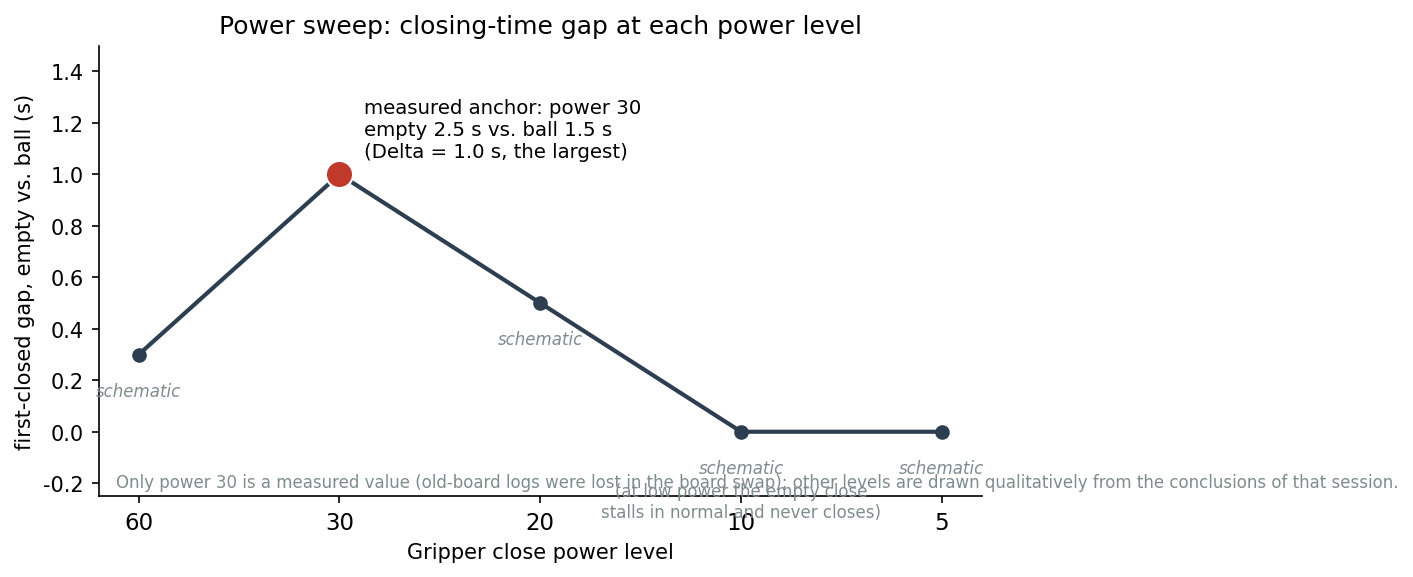
\includegraphics[width=0.88\linewidth]{figures/fig3_power_sweep.png}
\caption{Closing-time gap between empty and ball closes at each power level. Only power 30 is a measured value (old-board logs were lost in the board swap); the other levels are drawn qualitatively from that session's conclusions}
\label{fig:sweep}
\end{figure}

\section{The Final Rules}

\subsection{Four Branch Rules}
Let $t$ be the time from the close command to the first observation of
\texttt{closed}:

\begin{center}
\small
\begin{tabular}{p{5.2cm}p{3.4cm}p{6.2cm}}
\toprule
Observation & Action & Interpretation \\
\midrule
first \texttt{closed}, $t \le 2.0$ s & accept & stopped by the object before bottoming out (ball measured 1.5 s) \\
first \texttt{closed}, $t > 2.0$ s & reject & ran to the mechanical limit, treated as empty (empty measured 2.5 s) \\
\texttt{normal} held 2.5 s with fresh messages & accept & covers a rigid object wedging the jaws at \texttt{normal} \\
no acceptable result within 8.0 s & reject & never continue or wait without evidence \\
\bottomrule
\end{tabular}
\end{center}

The decision flow is shown in Figure~\ref{fig:flow}. The core
implementation lives in \texttt{real/pick\_place\_lua\_params.py}, lines
152--212 (comments translated here; the code is unchanged):

\begin{lstlisting}[firstline=152,lastline=212]{}
def close_and_judge(gripper):
    """Close the gripper and judge whether an object was grasped.
    Returns (success, detail).

    Criteria come from the real-machine power-state sweep (GRIP_POWER=30):
      1. status reaches "closed" within GRIP_CLOSED_FAST (2.0s)
         -> jaws were stopped mid-travel -> object grasped
            (measured: tennis ball 1.5s)
      2. status reaches "closed" after GRIP_CLOSED_FAST
         -> jaws ran to the mechanical limit -> nothing grasped
            (measured: empty close 2.5s)
      3. status holds "normal" for GRIP_STABLE_TIME without ever
         reaching "closed"
         -> object wedges the jaws mid-way -> grasped
            (the rigid block takes this branch)
      4. timeout / no push -> undecidable -> fail

    Note: never pause() mid-close -- the jaws get frozen before the
    limit and the state would sit at "normal", fooling the judgment.
    """
    gripper_status["value"] = "unknown"
    gripper_status["ts"] = 0.0
    gripper.close(power=GRIP_POWER)

    t0 = time.time()
    deadline = t0 + GRIP_STATUS_TIMEOUT
    last = None
    stable_since = None

    while True:
        now = time.time()
        v = str(gripper_status["value"]).strip().lower()
        ts = gripper_status.get("ts", 0.0)

        # criteria 1/2: time to first "closed"
        if v == "closed":
            elapsed = now - t0
            if elapsed <= GRIP_CLOSED_FAST:
                return True, (
                    f"fast close ({elapsed:.1f}s <= {GRIP_CLOSED_FAST}s), "
                    f"grasped"
                )
            return False, (
                f"slow close ({elapsed:.1f}s > {GRIP_CLOSED_FAST}s), "
                f"ran to the limit, nothing grasped"
            )

        # criterion 3: "normal" held steadily (push must still flow)
        if v != last:
            last = v
            stable_since = now
        elif (v == "normal" and stable_since is not None
              and now - stable_since >= GRIP_STABLE_TIME
              and ts > 0 and now - ts < 1.0):
            return True, (
                f"jaws steadily held mid-way at normal"
                f"({GRIP_STABLE_TIME}s), grasped"
            )

        if now >= deadline:
            return False, (
                f"timeout ({GRIP_STATUS_TIMEOUT}s) with no stable verdict, "
                f"last state {gripper_status['value']}"
            )

        time.sleep(0.2)
\end{lstlisting}

\begin{figure}[htbp]
\centering
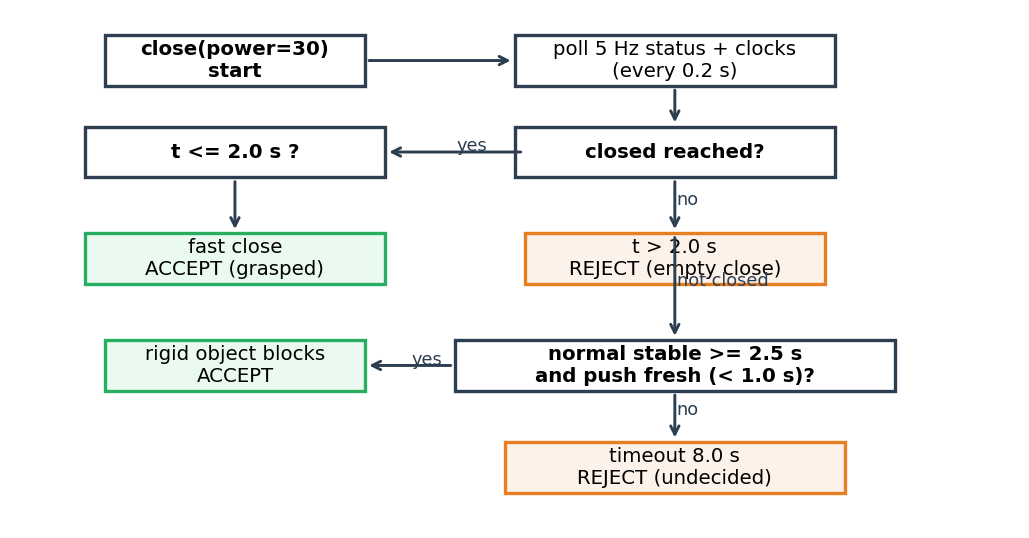
\includegraphics[width=0.9\linewidth]{figures/fig5_flow.png}
\caption{Decision flow of close\_and\_judge}
\label{fig:flow}
\end{figure}

\subsection{What These Numbers Are}
Three things need to be said plainly. First, $t$ is the delay from the close
command to the first observed \texttt{closed}, not some absolute time.
Second, the status subscription runs at 5\,Hz and the program polls every
0.2\,s, so the observation granularity is about 0.2\,s. Third, these
thresholds are empirical values for the current object (a tennis ball) and
the current scene, backed by the sweep data --- not a general semantics of
the SDK state machine. Any new object requires a fresh sweep and fresh
parameters; Appendix B shows one such re-sweep.

\section{Five Acceptance Runs}

The acceptance test ran on 11 September. The five rounds (logs saved to the
desktop as \texttt{test\_<timestamp>.txt}; commit \texttt{d5f8c04} attaches
the acceptance video and logs):

\begin{center}
\small
\begin{tabular}{cccccc}
\toprule
Round & Ground truth & Closing observation (s) & Judgment & What followed \\
\midrule
1 & object & 1.4 & accept & carried through \\
2 & object & 1.4 & accept & carried through \\
3 & object & 1.6 & accept & carried through \\
4 & object & 1.4 & accept & carried through \\
5 & empty (planned) & 2.4 & reject & cycle stopped, safe return \\
\bottomrule
\end{tabular}
\end{center}

\begin{figure}[htbp]
\centering
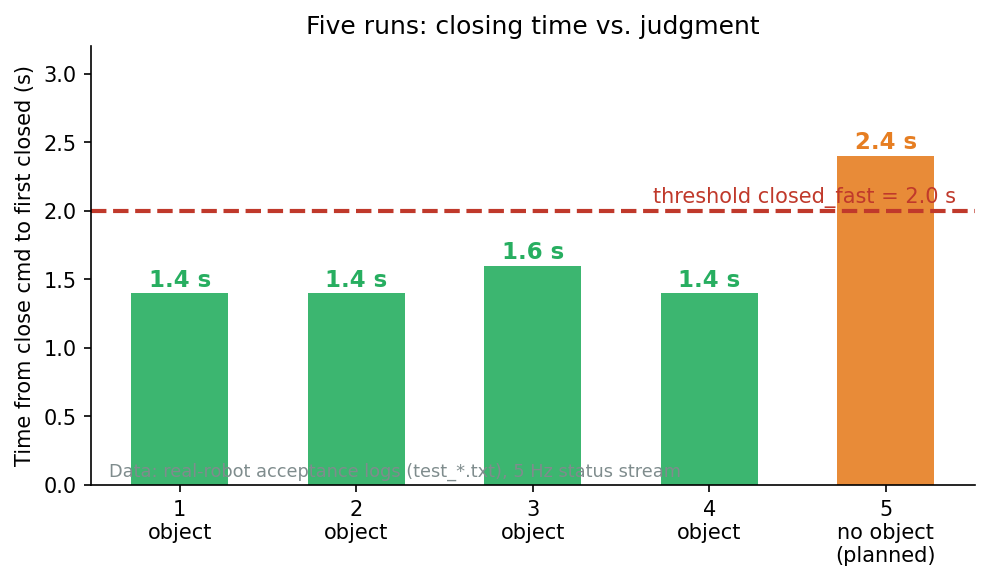
\includegraphics[width=0.85\linewidth]{figures/fig2_close_times.png}
\caption{Closing times of the five runs against the 2.0 s threshold}
\label{fig:times}
\end{figure}

I report the results in two subsets: object-present 4/4 accepted and carried
through; the deliberate empty close 1/1 correctly rejected. The program's raw
count is 4/5 --- round 5 was a planned negative case (no object placed, to
exercise the empty-close failure branch), not a failed grasp, so it must not
be folded into an ``80\% success rate''. The mean closing time of the four
object runs is 1.45\,s.

One sentence about the threshold margin, to be honest: the fastest object run
(1.6\,s) and the empty close (2.4\,s) are both exactly 0.4\,s away from the
2.0\,s threshold, but with 5\,Hz pushes and 0.2\,s polling the observation
granularity is about 0.2\,s, and communication and scheduling add more
uncertainty --- so the 0.4\,s only says the two cases separated cleanly in
this batch; it is not a strict error margin.

\begin{figure}[htbp]
\centering
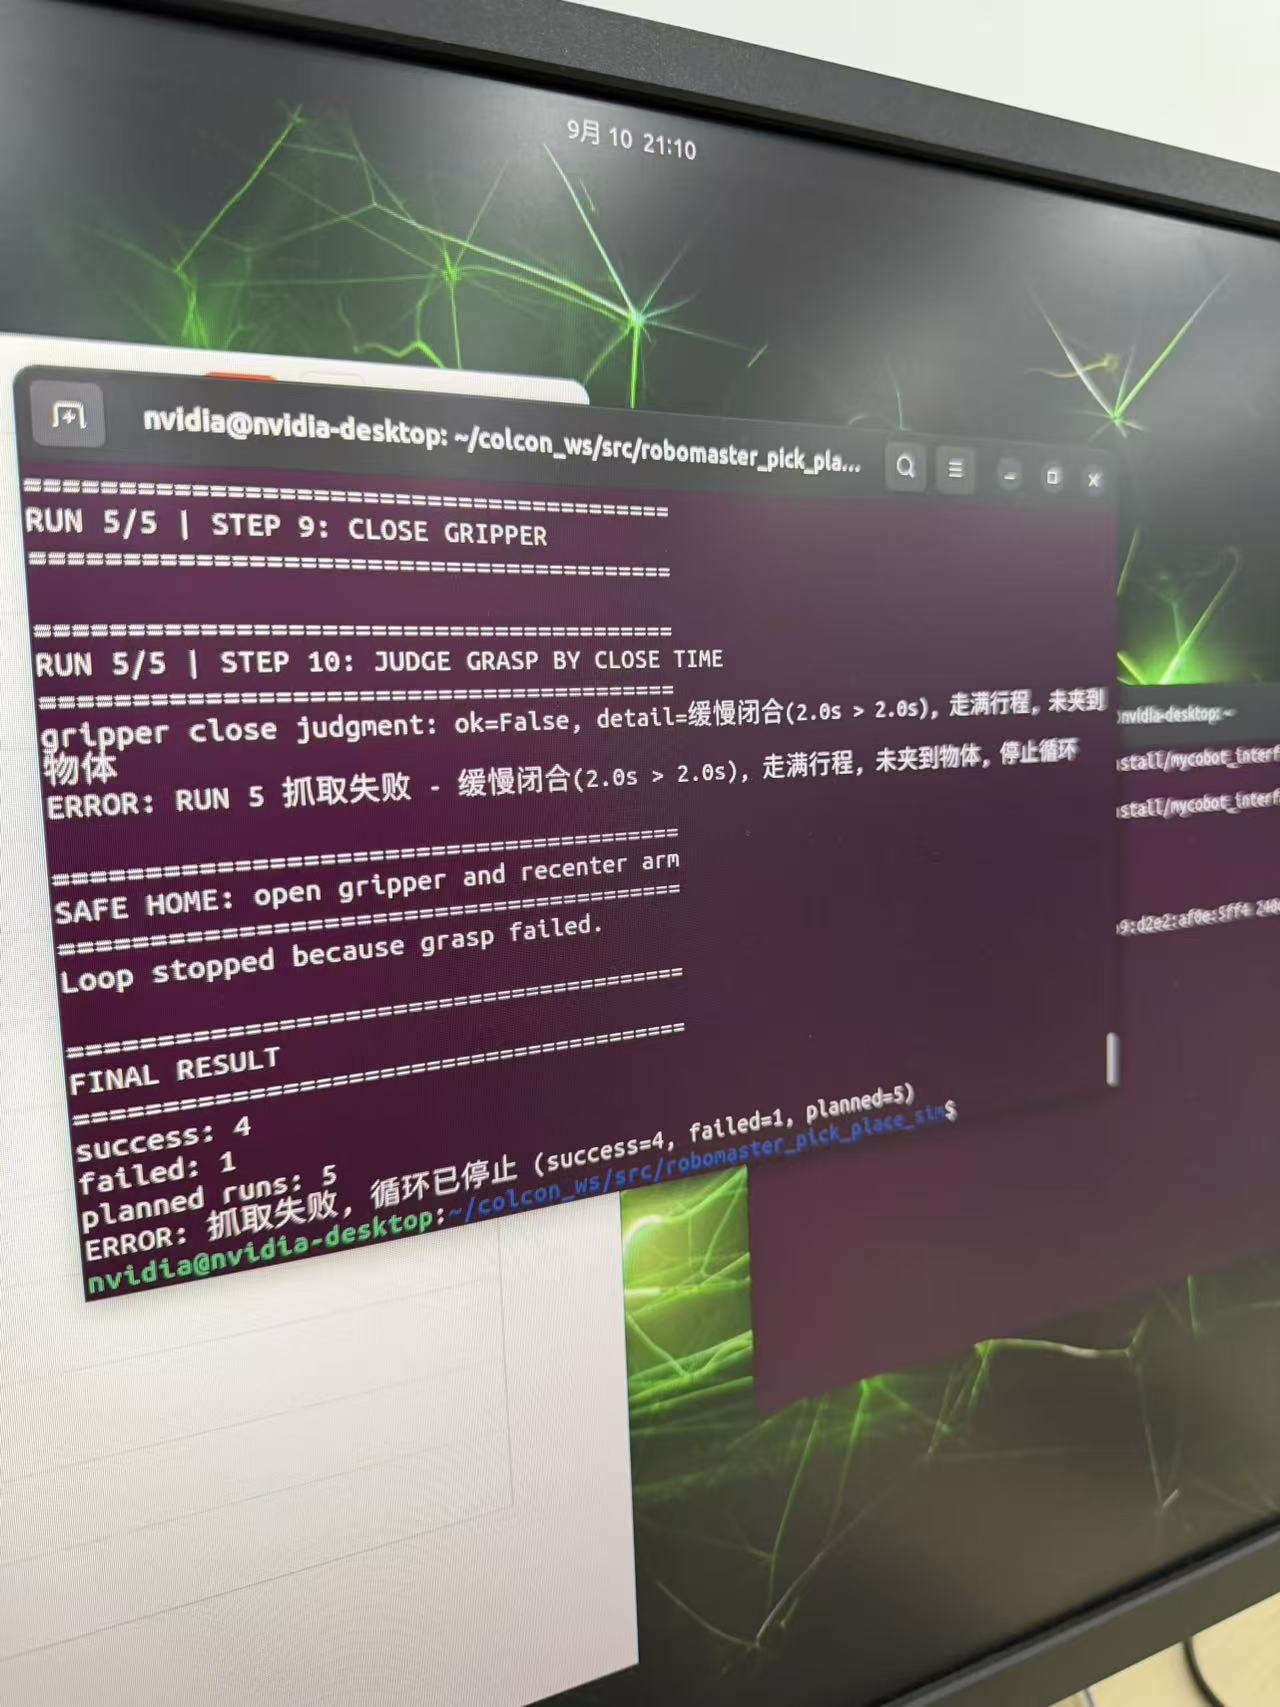
\includegraphics[width=0.55\linewidth]{photos/p2.jpg}
\caption{Gripper holding a tennis ball}
\label{fig:grip}
\end{figure}

\begin{figure}[htbp]
\centering
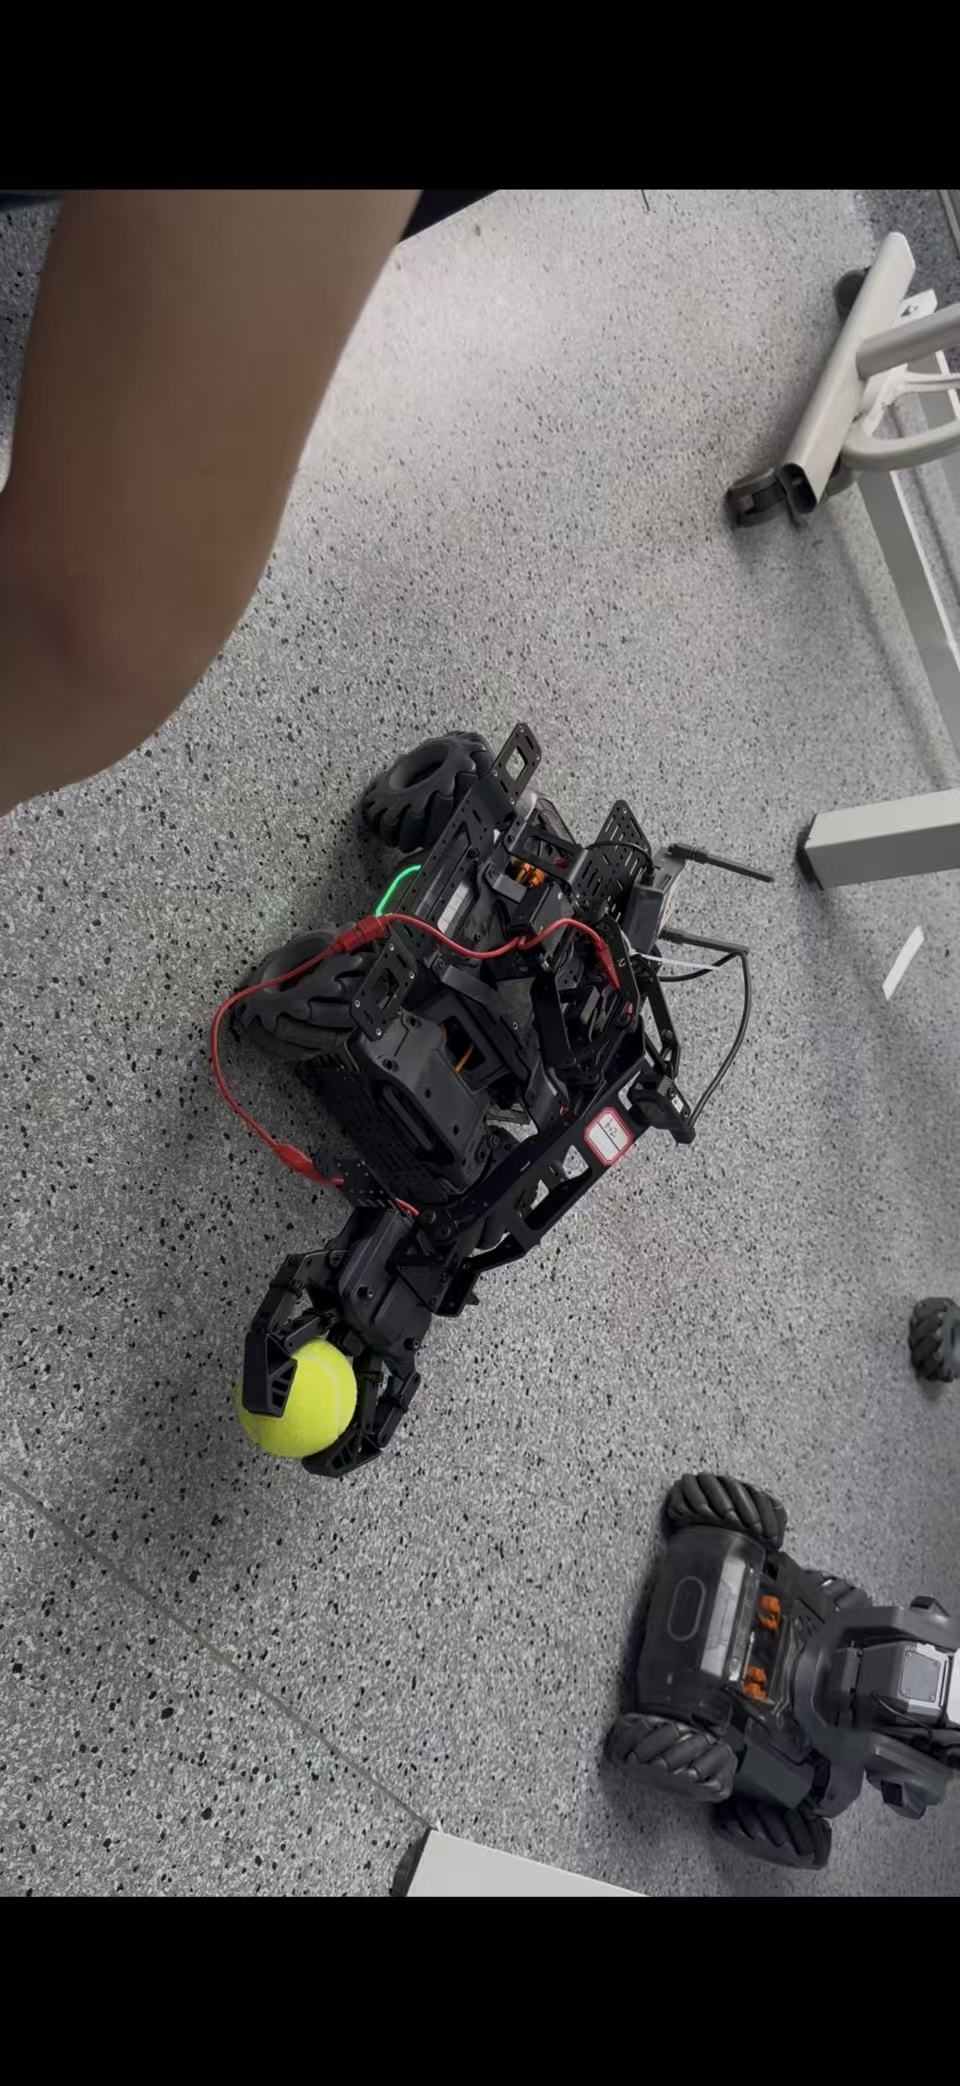
\includegraphics[width=0.6\linewidth]{photos/p3.jpg}
\caption{Acceptance run log}
\label{fig:log1}
\end{figure}

\section{Hand-off to the Motion Pipeline}

\texttt{close\_and\_judge} returns (continue?, reason) and is consumed by
Gong Chengtian's real-robot motion module. On accept it runs the test lift
(+25\,mm), main lift (+60\,mm), turn to B ($-180^\circ$, 20\,$^\circ$/s),
lower 80\,mm, release and withdraw; on reject it stops the cycle, raises the
alarm signal (armor LEDs flashing red plus an alarm sound, function
\texttt{robot\_signal\_error}), opens the gripper and attempts to re-center
(\texttt{safe\_home}). Round 5 exercised the reject path end to end: the
module returned ``slow close'' at 2.4\,s and rejected, the chain stopped
without executing any carry motion, and the arm then returned safely.

\begin{figure}[htbp]
\centering
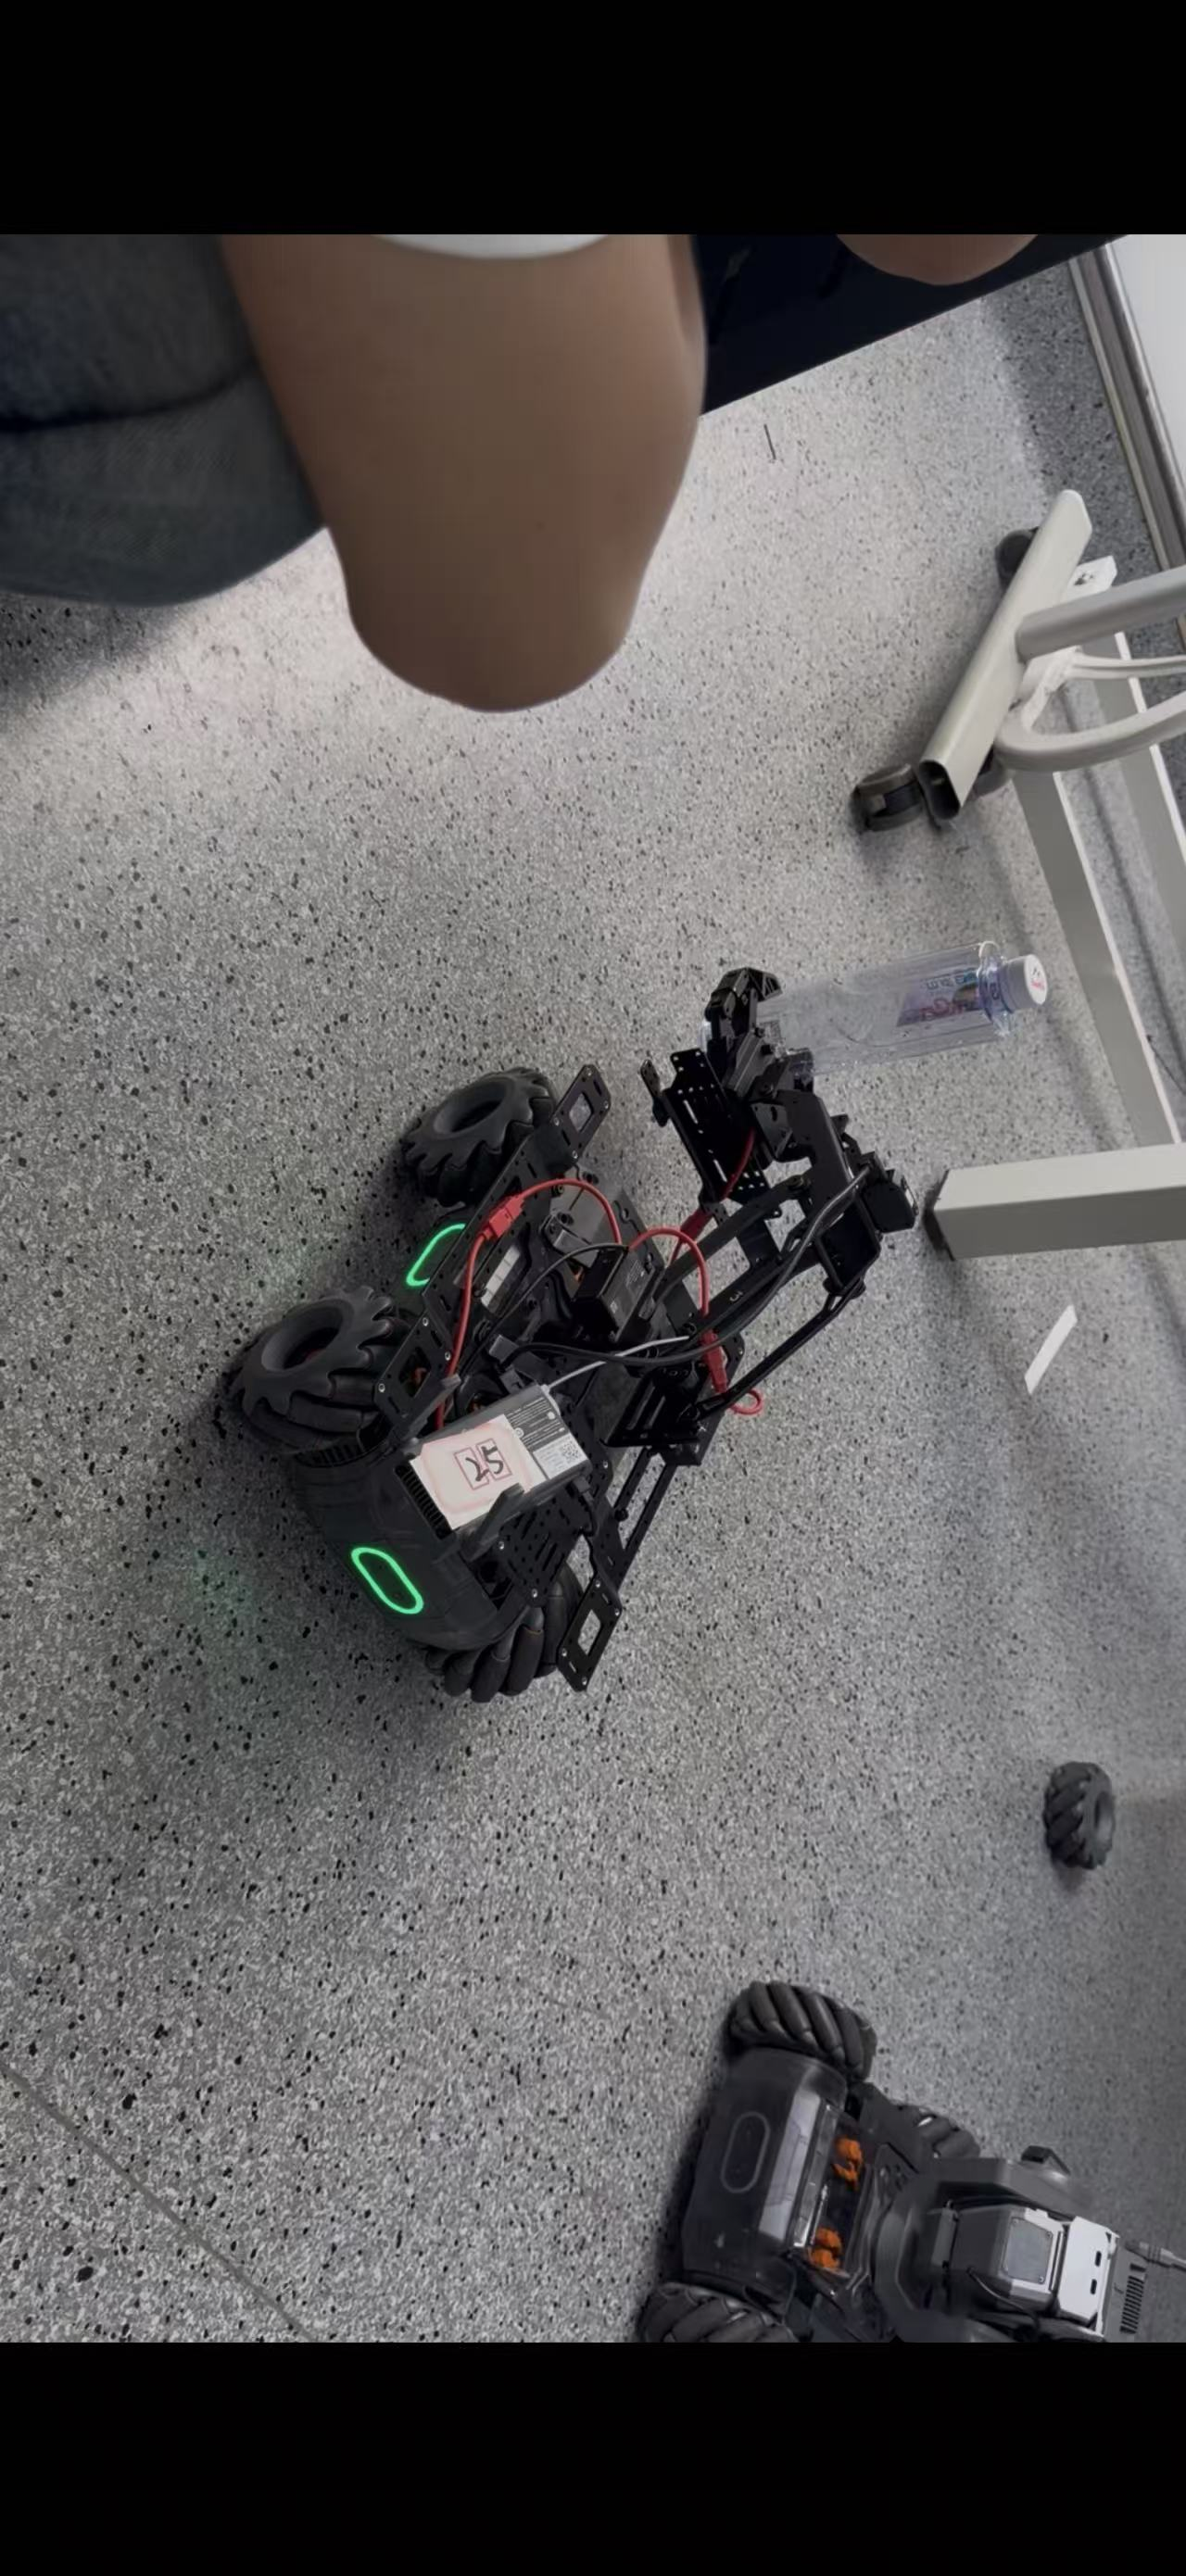
\includegraphics[width=0.55\linewidth]{photos/p4.jpg}
\caption{Terminal output of the round-5 empty-close rejection}
\label{fig:log2}
\end{figure}

\begin{figure}[htbp]
\centering
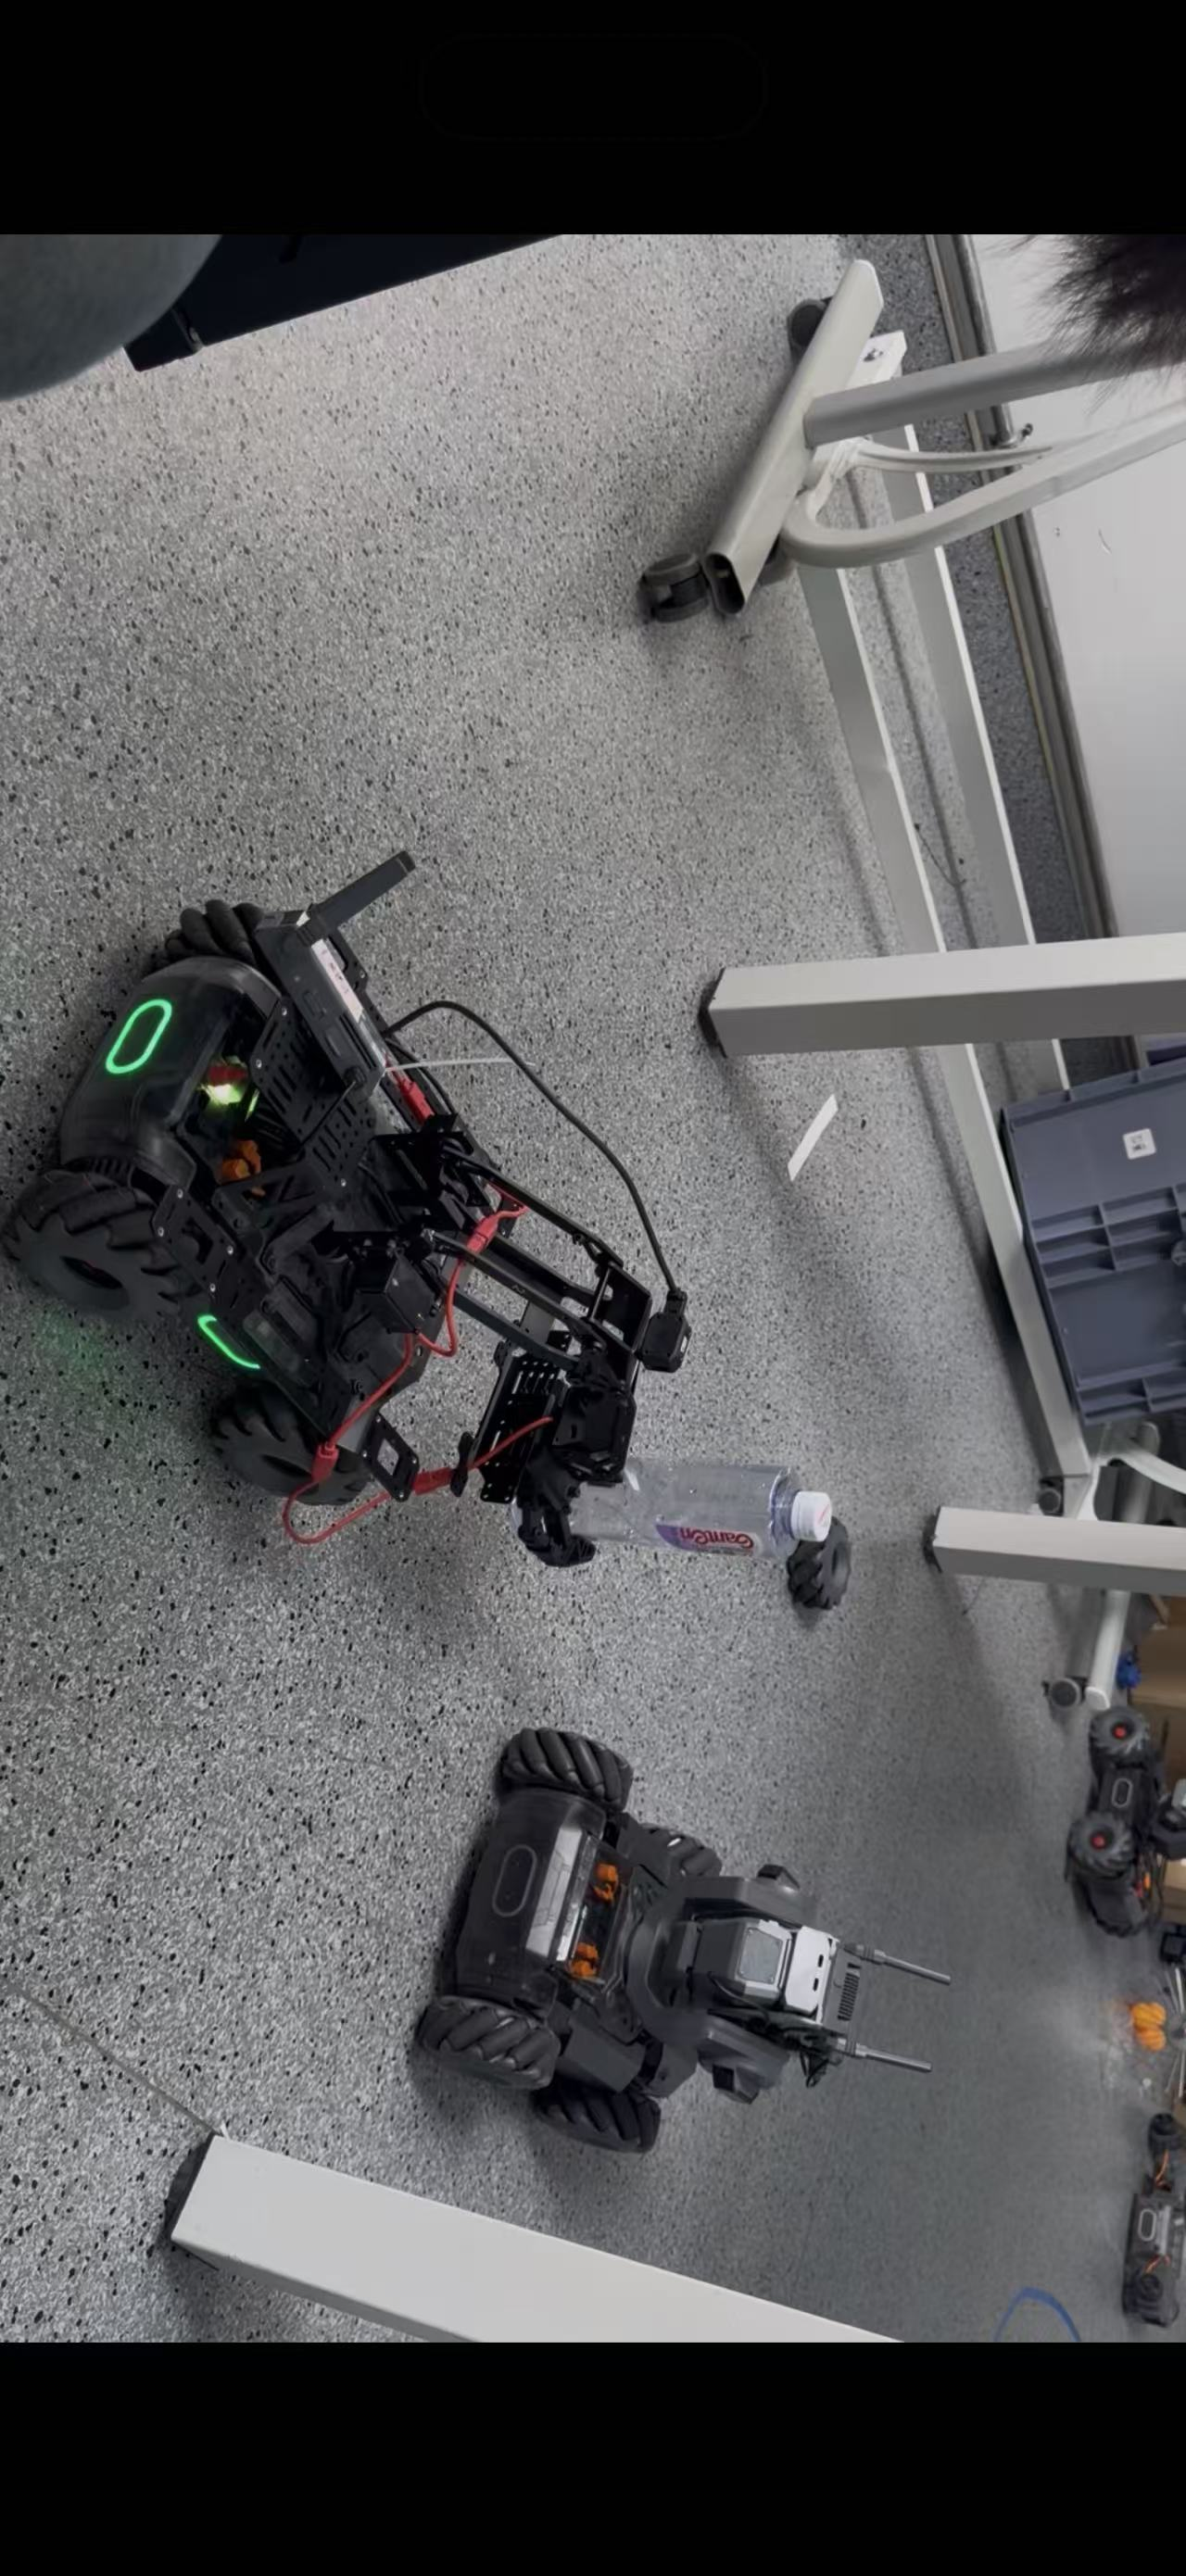
\includegraphics[width=0.55\linewidth]{photos/p5.jpg}
\caption{On-site record from the acceptance runs}
\label{fig:log3}
\end{figure}

\begin{figure}[htbp]
\centering
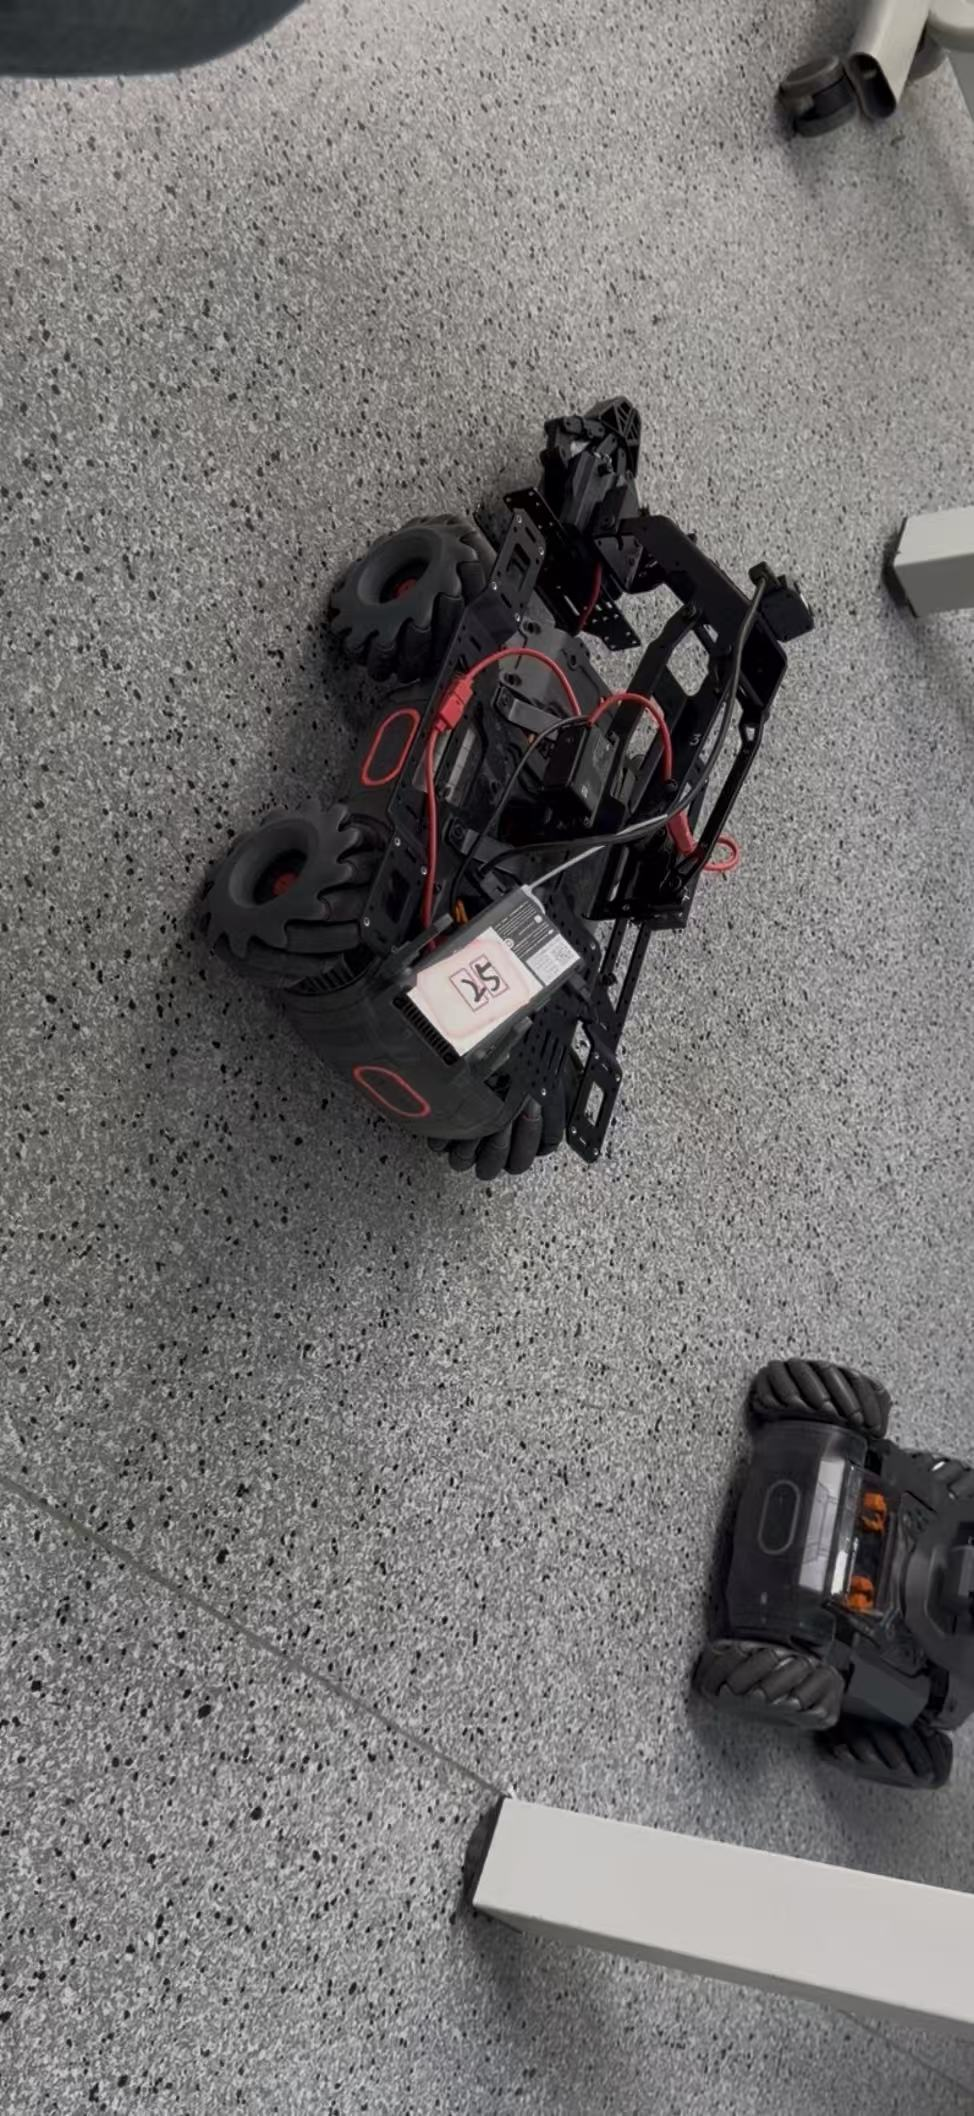
\includegraphics[width=0.55\linewidth]{photos/p6.jpg}
\caption{On-site record from the acceptance runs (continued)}
\label{fig:log4}
\end{figure}

\begin{figure}[htbp]
\centering
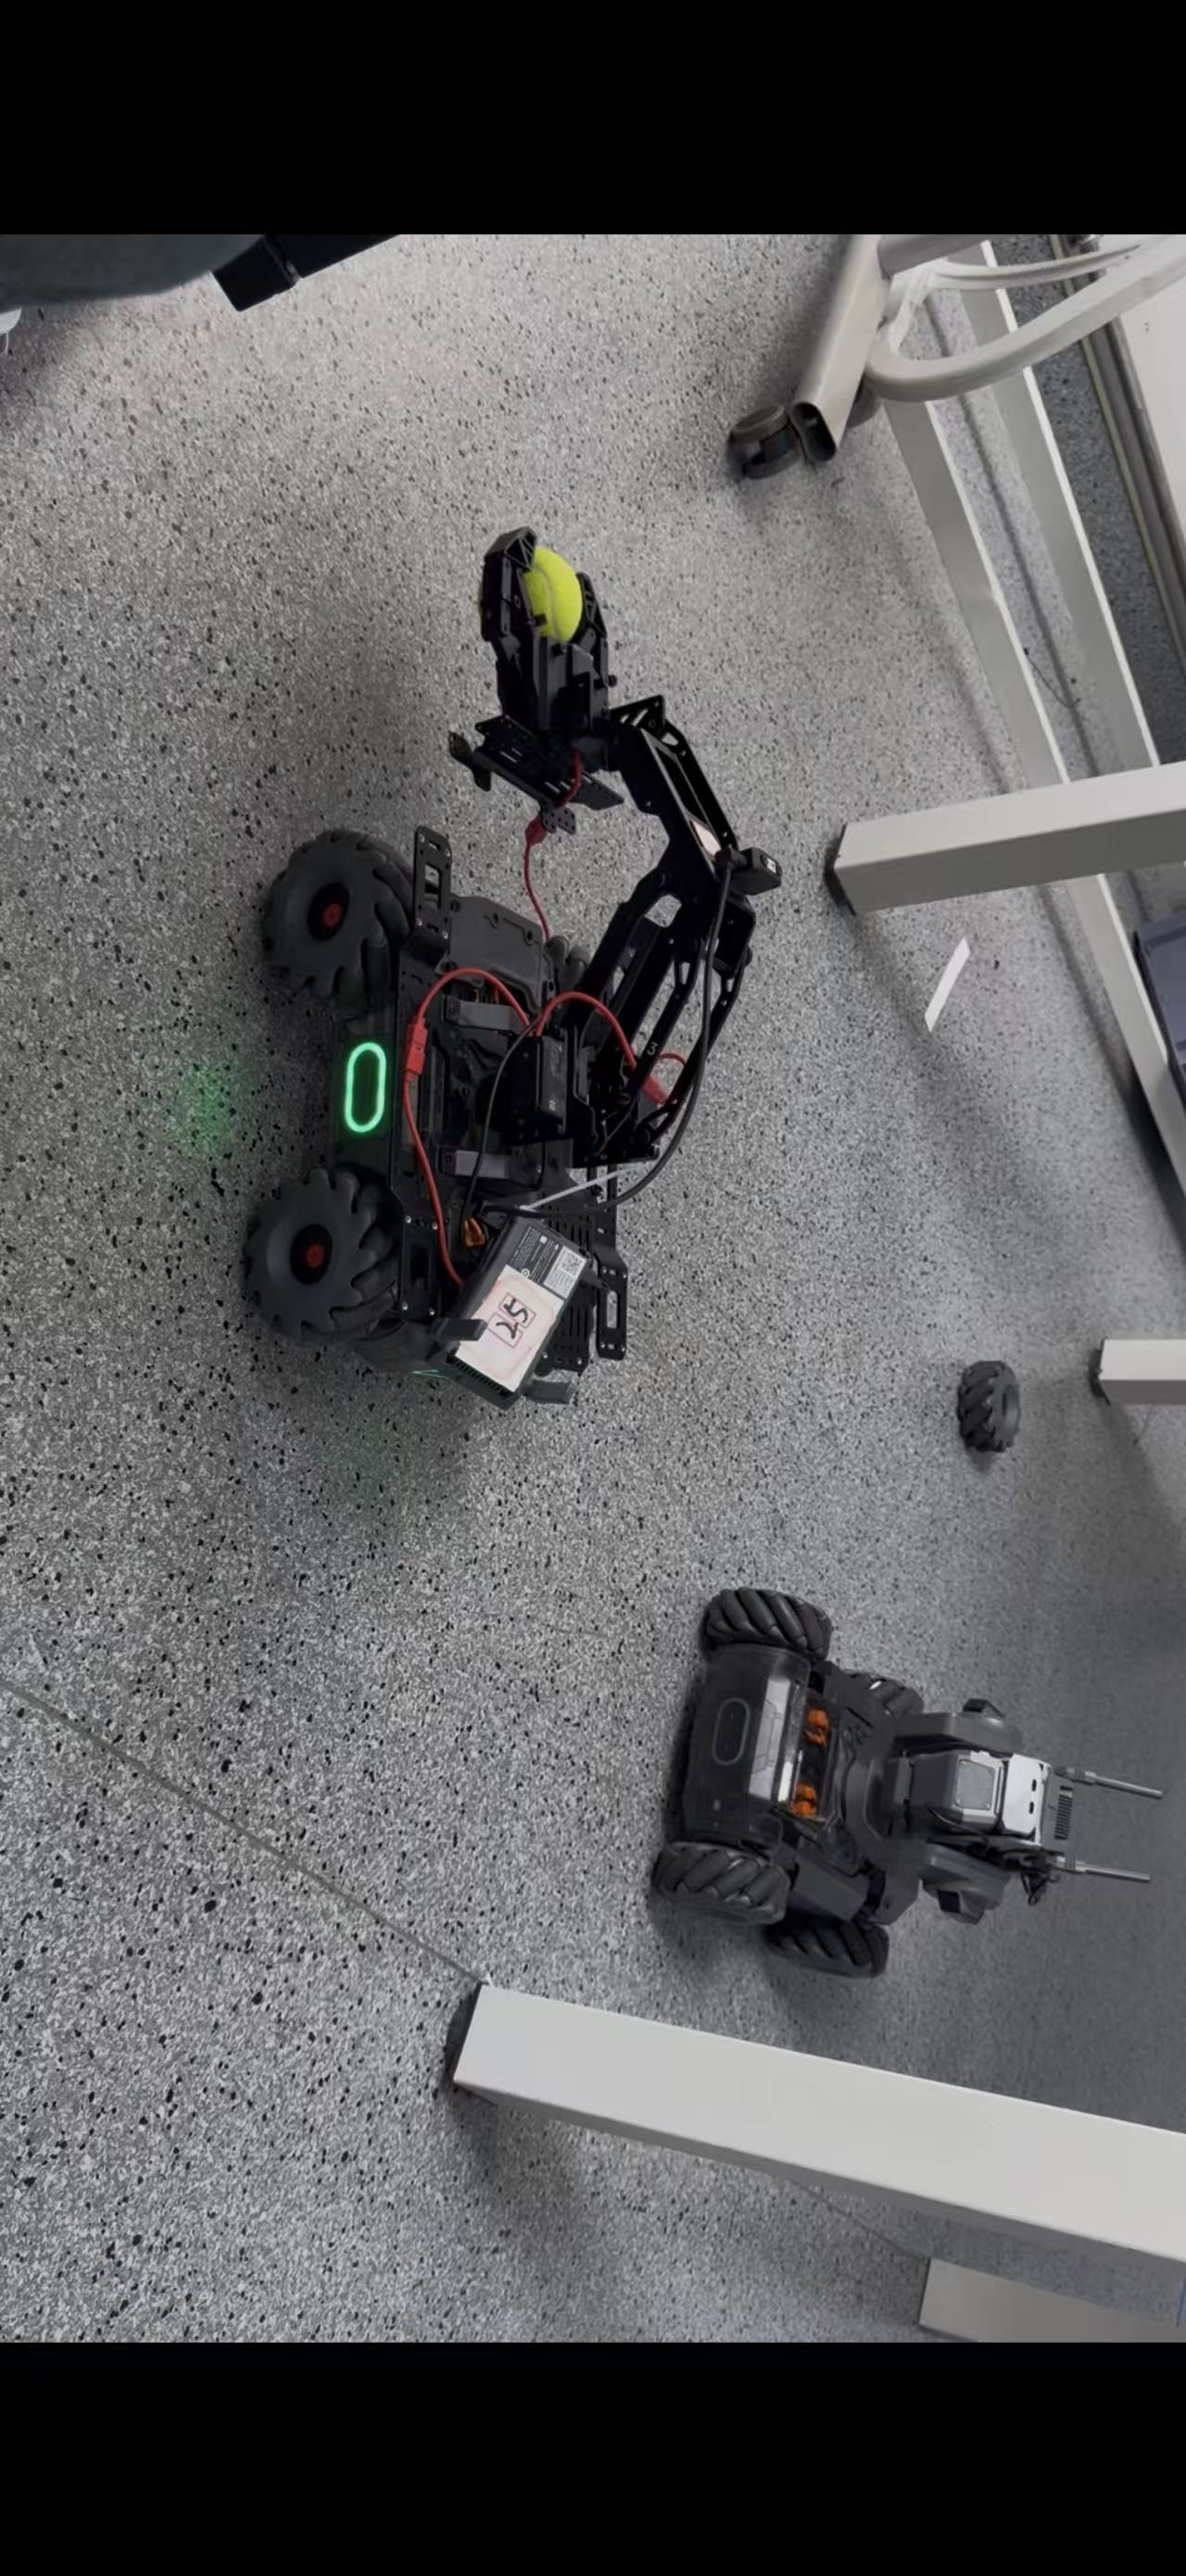
\includegraphics[width=0.55\linewidth]{photos/p7.jpg}
\caption{Record of the safe return procedure}
\label{fig:log5}
\end{figure}

One more thing to state clearly: whether the object actually rides up with
the jaws after the test lift is still confirmed by eye on site --- the module
has no visual or force feedback loop. It answers ``does this round satisfy
the criterion'', not ``did the object land in B''.

\section{Evaluation and Limitations}

Judgment accuracy needs an independent ground truth plus four counts (true
positive, true negative, false accept, false reject); with four positive and
one negative sample there is no statistically meaningful accuracy to report,
only ``the two cases separated correctly in this batch''. Carry success also
involves motion execution, holding, turning, release and landing, none of
which gripper verification alone can vouch for. Power 30 has the best time
separation in this calibration, but that says nothing about other object
stiffnesses or battery levels; any new object needs its own sweep
(Appendix B).

The main shortcoming is that no communication-failure test was done by
injection. When the gripper status subscription dies, criterion 3 stops
accepting because freshness expires --- that part of the logic is correct ---
but the rest of the wait logic was never exercised against a dead link, and
every round so far ran on a healthy one. There is no guarantee that
``software homing'' still works when the link is down; safe recovery might
depend on manually cutting power. The next step is a failure-injection test,
keeping the physical emergency stop / power cut and the software homing as
two independent measures, with the pass criterion: after an injected link
loss the robot times out on schedule, enters a safe state, and makes no
uncontrolled motion.

\section{Conclusion}

What the module ended up being is not complicated: a 5\,Hz status stream,
0.2\,s polling, a 2.0\,s closing-time threshold, a 2.5\,s stable window, an
8.0\,s total timeout, and two separate clocks. But every one of those pieces
was pushed out by a specific misjudgment on the real robot, not designed up
front. Acceptance results: all four object runs closed within 1.6\,s, were
accepted, and were carried through; the deliberate empty close was rejected
at 2.4\,s, the cycle stopped, and the arm returned safely --- at no point did
the robot carry on with empty jaws. The sample size and object variety are
limited; the generality of this criterion and its behavior under failure
scenarios still need more batches and dedicated fault testing.

\appendix
\section{My Git History}
This is my complete commit history in the project repository
\texttt{robomaster\_pick\_place\_sim} (branch
\texttt{codex/jetson-dji-real-test}), 54 commits in total. The ones related
to the verification module cluster between 18:39 and 21:00 on 10 September
and on acceptance day, 11 September; every hash cited in the main text can be
found here. Commit messages are quoted as recorded in the repository (most
are in Chinese).

\begin{center}
\footnotesize
\begin{longtable}{p{2.2cm}p{2.2cm}p{10.4cm}}
\toprule
Hash & Date & Message \\
\midrule
\endhead
% auto-generated from git log --author=LpTriX
\texttt{45abec9} & 09-13 20:30 & vision: bottle 扫参判读 (规则2) → power=20, closed\_fast=2.0 \\
\texttt{39f6143} & 09-13 06:37 & vision: 移交 README 记录二轮 dry-run 结果 + 有效带下限待观察项 \\
\texttt{49a542f} & 09-13 06:17 & vision: 视觉联动定点抓取 (calibrate.py + vision\_pick\_place.py) + 移交 README \\
\texttt{c94d34e} & 09-13 03:59 & vision: FP16 定为默认验收引擎 (实机 A/B 确认效果更好) \\
\texttt{3c49f23} & 09-13 03:53 & vision: README 记录 FP16 实测 29.7ms \\
\texttt{86b5354} & 09-13 03:51 & vision: README 记录真机实测数据 (FP32 \~\{\}70ms, conf 0.83-0.94) \\
\texttt{d8091e9} & 09-13 03:39 & vision: fix log-line fps (was cumulative-count/2s, not a rate) \\
\texttt{230522e} & 09-13 03:37 & vision: fix FPS display stuck at 0.00 (ms-\textgreater{}fps unit conversion) \\
\texttt{584674b} & 09-13 03:34 & vision: 视觉检测节点 (SDK 相机 + TRT YOLOv8s) 部署全流程 \\
\texttt{667923d} & 09-13 02:32 & real: add camera pipeline debug scripts \\
\texttt{545aea7} & 09-13 02:18 & real: throttle Empty-exception spam when stream stalls \\
\texttt{1e05efc} & 09-13 02:11 & real: window-first viewer, selftest mode, strip ROS env, fix tee whitespace \\
\texttt{e00a82a} & 09-13 01:57 & real: retry SDK init 3x for flaky robot WiFi \\
\texttt{fb4ba67} & 09-13 01:54 & real: live-flush tee log + os.\_exit to survive SDK shutdown hangs \\
\texttt{3717d36} & 09-13 01:44 & real: text-SDK fallback on SDK init failure; update AP hint to new controller SSID \\
\texttt{5141e14} & 09-13 01:21 & real: camera\_viewer v2 main-thread display + watchdog cleanup (SDK stop/close hangs) \\
\texttt{9330fbf} & 09-13 00:59 & real: live-stream diagnostic + Team21 paths, socket spy patches methods not the socket class \\
\texttt{e90c18e} & 09-11 17:00 & real: H264 decoder assign pts to parsed packets (PyAV 17 reorder buffer fix) \\
\texttt{3659fbe} & 09-11 16:48 & real: live camera viewer with PyAV H264 decoder \\
\texttt{d5f8c04} & 09-11 15:11 & exp2: real robot acceptance video and run log (4/5 passed) \\
\texttt{422513c} & 09-11 14:45 & real: name desktop run logs test\_\textless{}timestamp\textgreater{}.txt \\
\texttt{20d9356} & 09-10 21:21 & real: desktop run logs, acceptance line, package ROS2 node \\
\texttt{7ecd31d} & 09-10 21:00 & gripper judgment: decide by close time (tennis ball fix) \\
\texttt{79f9dbb} & 09-10 20:48 & real: 主脚本参数非法时给出友好提示而不是裸崩 \\
\texttt{b20ee4e} & 09-10 20:42 & real: 扫描探针无论成败都保存日志到桌面 \\
\texttt{a9d6afc} & 09-10 20:26 & real: 扫描探针输出保存到桌面, 带标记和时间戳文件名 \\
\texttt{8d6548c} & 09-10 20:23 & real: 新增功率-状态扫描探针 (网球调试) \\
\texttt{e306600} & 09-10 20:10 & real: 探针支持指定闭合功率, 主脚本支持命令行覆盖 GRIP\_POWER \\
\texttt{dd14b7f} & 09-10 19:53 & fix(real): 判定改为稳定窗口, 修复空夹中途 normal 的竞态误判 \\
\texttt{86d2162} & 09-10 19:41 & real: probe 增加 WiFi 预检, 未连机器人热点时给出明确提示 \\
\texttt{907c028} & 09-10 19:32 & fix(real): poll gripper status instead of pausing mid-close \\
\texttt{d5a6e71} & 09-10 19:12 & real: README 补充 libmedia\_codec 存根一次性配置 (aarch64 无 .so) \\
\texttt{4079d1c} & 09-10 19:03 & real: 改用 pip 安装的官方 SDK, 移除 \~\{\}/RoboMaster-SDK/src 路径注入 \\
\texttt{6f5b743} & 09-10 18:39 & real: 夹爪完全闭合判定 + 机器人端报错/报成功显示 \\
\texttt{5f7fa1f} & 09-10 16:14 & lpx: 机械臂定点抓取完整方案 — 仿真 MoveIt 抓取 + EP 真机驱动(伪装 ros2\_control) + 标定工具 + 真机手册 \\
\texttt{f019182} & 09-10 16:10 & docs: libmedia\_codec 存根修正 — LiveView 会实例化 H264Decoder/OpusDecoder, 存根需含空类 \\
\texttt{8cd6787} & 09-10 13:13 & 驱动退出清理 + runbook 更新为板上实际部署步骤 (ep\_ws 布局/符号链接/site-packages 存根) \\
\texttt{ea1fb71} & 09-10 12:51 & 真机驱动包: EP SDK 驱动伪装 ros2\_control 接口 + 标定工具 + 真机 launch/参数/手册 \\
\texttt{298865c} & 09-09 22:19 & 重构规划: 解析逆解+关节目标替代 OMPL 路径约束; 重标定 4 个预设点 \\
\texttt{98d6387} & 09-09 21:53 & 修复联调第二批问题: meshes 未安装 + ACM 字段名/语义错误 \\
\texttt{7c4701b} & 09-09 21:50 & 修复验收联调三处问题 + 视觉升级: 官方 mesh 移植进 URDF \\
\texttt{0d27eea} & 09-09 21:24 & 修复抓取几何: home 位姿上仰避障 + 可达性驱动的抓取流程重写 \\
\texttt{3ec7144} & 09-09 21:07 & 修复 move\_group 参数结构: planning\_pipelines 列表 + 标准控制器配置 + 轨迹执行改用 Action \\
\texttt{0ac2aad} & 09-09 20:46 & 修复: move\_group.launch.py 的 robot\_description 同样用 ParameterValue(str) 包裹 \\
\texttt{aa1d9fd} & 09-09 20:42 & 修复: launch 文件中 robot\_description 用 ParameterValue(value\_type=str) 包裹 \\
\texttt{ceefa5e} & 09-09 20:34 & 修复: 补充 setup.cfg 把 console\_scripts 装到 lib/\textless{}pkg\textgreater{} (ament\_python 惯例) \\
\texttt{e2bcdb3} & 09-09 20:30 & 重构: 抓取节点改用 MoveIt 原生接口, 去掉 moveit\_commander 依赖 \\
\texttt{ea8409b} & 09-09 17:24 & 文档: README 使用指南 + .gitignore \\
\texttt{c5b3dbc} & 09-09 17:23 & 新增: MoveIt 抓取节点与辅助脚本 \\
\texttt{5fae9b7} & 09-09 17:18 & 新增: 一体化 launch 一键启动 Gazebo + MoveIt + 抓取任务 \\
\texttt{fdd4858} & 09-09 17:18 & 新增: MoveIt 配置包 robomaster\_ep\_moveit\_config \\
\texttt{0475f3d} & 09-09 17:16 & 新增: 仿真世界中加入桌面、A/B 标记和目标物体 \\
\texttt{231a1ee} & 09-09 17:15 & 新增: 底盘偏航关节 base\_yaw\_joint, 工作空间扩展为桌面圆环区域 \\
\texttt{152edaa} & 09-09 17:14 & 修复: 控制器配置路径参数化为 \$(find), launch 改用 spawner 加载控制器 \\
% end
\bottomrule

\end{longtable}
\end{center}

\section{Reusing the Sweep Tool on a Bottle (2026-09-13)}
When the team later upgraded to vision-guided picking, I re-ran the same
sweep tool on a bottle (a rigid object), once empty and once with the bottle
held in the jaws; the first-closed times are in Table~\ref{tab:bottle}. No
power level showed the ``empty closes but bottle never closes'' pattern: at
every level that closes at all, the bottle also closes. Applying the rule
``take the level with the largest time gap, threshold at the midpoint''
picked power 20 with a 2.0\,s threshold. This instance makes two points: the
sweep workflow transfers to new objects, and the parameters must be re-swept
per object rather than inherited.

\begin{table}[htbp]
\centering
\small
\begin{tabular}{cccc}
\toprule
Power level & Empty, first closed & Bottle, first closed & Gap \\
\midrule
60 & 2.5 s & 2.0 s & 0.5 s \\
30 & 2.0 s & 1.5 s & 0.5 s \\
20 & 2.5 s & 1.5 s & 1.0 s (largest) \\
10 & not closed within 8 s & not closed within 8 s & indistinguishable \\
5 & not closed within 8 s & not closed within 8 s & indistinguishable \\
\bottomrule
\end{tabular}
\caption{Bottle sweep summary (logs: \texttt{~/Desktop/}\allowbreak
\texttt{gripper\_sweep\_bottle\_empty\_20260913\_063403.txt} and
\texttt{gripper\_sweep\_bottle\_20260913\_063527.txt})}
\label{tab:bottle}
\end{table}

\begin{figure}[htbp]
\centering
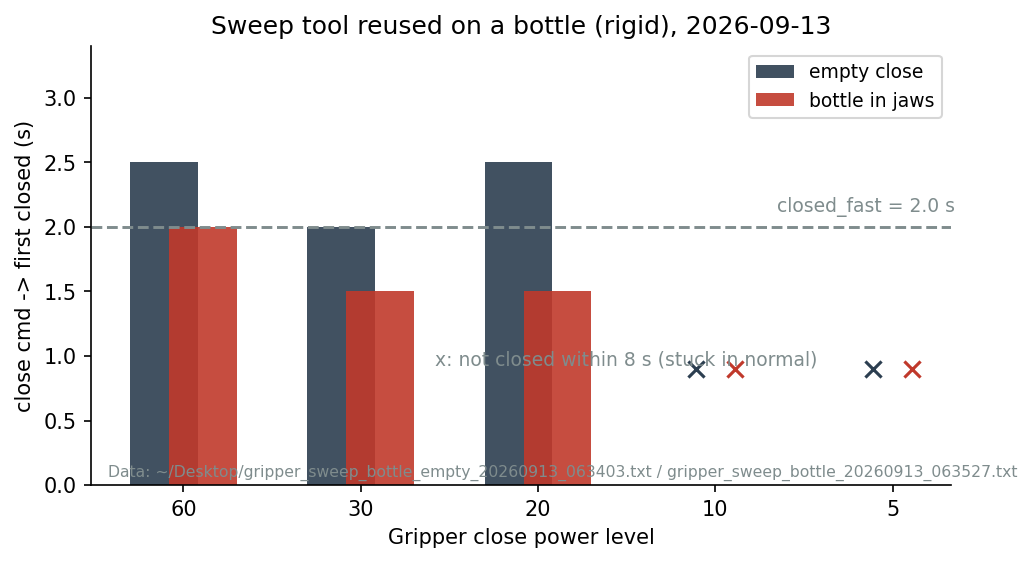
\includegraphics[width=0.85\linewidth]{figures/fig6_bottle_sweep.png}
\caption{Measured data from reusing the sweep tool on a bottle}
\label{fig:bottle}
\end{figure}

One observation worth recording: the bottle, rigid as it is, ended up in
\texttt{closed} rather than stuck at \texttt{normal} at these power levels,
so the \texttt{normal}-stable branch of Section 3.3 still has never fired on
the real robot. A dedicated test for that branch is worth adding later.

\section{Code and File Index}

\begin{center}
\small
\begin{tabular}{p{4.6cm}p{2.4cm}p{8.0cm}}
\toprule
File & Lines & Content \\
\midrule
\texttt{real/pick\_place\_lua\_params.py} & L30--41 & judgment parameters (power / thresholds / timeout) \\
\texttt{real/pick\_place\_lua\_params.py} & L152--212 & \texttt{close\_and\_judge} implementation \\
\texttt{real/pick\_place\_lua\_params.py} & L215--236 & \texttt{safe\_home} safe return \\
\texttt{real/pick\_place\_lua\_params.py} & L239--252 & \texttt{robot\_signal\_error} alarm signal \\
\texttt{real/gripper\_status\_sweep.py} & whole file & power sweep probe (60/30/20/10/5) \\
\texttt{vision/vision\_pick\_place.py} & parameterized reuse & per-class reuse of the same criterion in the vision task \\
\bottomrule
\end{tabular}
\end{center}

\end{document}
